\documentclass{standalone}
\usepackage{tikz}
\usetikzlibrary{patterns, positioning}


\begin{document}
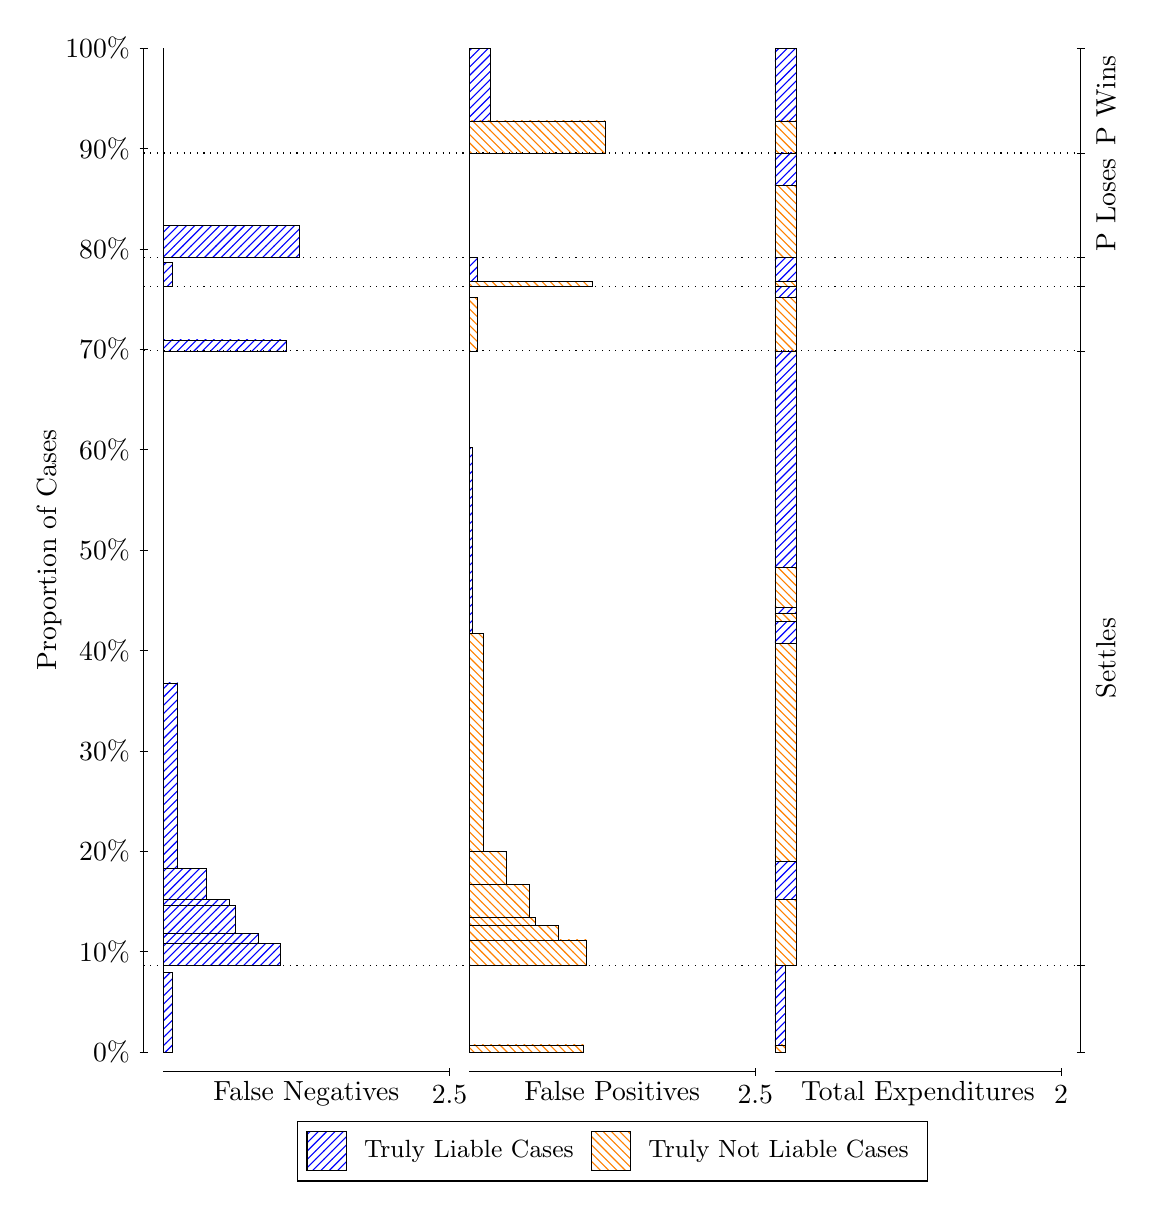
\begin{tikzpicture}
\draw[black, very thin] (1.5,1.75) -- (1.5,14.5);
\node[rotate=90, text=black, anchor=center] at (0.3, 8.125) {Proportion of Cases};
\draw[black, very thin] (1.45,1.75) -- (1.55,1.75);
\node[text=black, anchor=east] at (1.45, 1.75) {0\%};
\draw[black, very thin] (1.45,3.025) -- (1.55,3.025);
\node[text=black, anchor=east] at (1.45, 3.025) {10\%};
\draw[black, very thin] (1.45,4.3) -- (1.55,4.3);
\node[text=black, anchor=east] at (1.45, 4.3) {20\%};
\draw[black, very thin] (1.45,5.575) -- (1.55,5.575);
\node[text=black, anchor=east] at (1.45, 5.575) {30\%};
\draw[black, very thin] (1.45,6.85) -- (1.55,6.85);
\node[text=black, anchor=east] at (1.45, 6.85) {40\%};
\draw[black, very thin] (1.45,8.125) -- (1.55,8.125);
\node[text=black, anchor=east] at (1.45, 8.125) {50\%};
\draw[black, very thin] (1.45,9.4) -- (1.55,9.4);
\node[text=black, anchor=east] at (1.45, 9.4) {60\%};
\draw[black, very thin] (1.45,10.675) -- (1.55,10.675);
\node[text=black, anchor=east] at (1.45, 10.675) {70\%};
\draw[black, very thin] (1.45,11.95) -- (1.55,11.95);
\node[text=black, anchor=east] at (1.45, 11.95) {80\%};
\draw[black, very thin] (1.45,13.225) -- (1.55,13.225);
\node[text=black, anchor=east] at (1.45, 13.225) {90\%};
\draw[black, very thin] (1.45,14.5) -- (1.55,14.5);
\node[text=black, anchor=east] at (1.45, 14.5) {100\%};

\draw[black, very thin] (13.4,1.75) -- (13.4,14.5);
\draw[black, very thin] (13.35,1.75) -- (13.45,1.75);
\node[anchor=west] at (13.35, 1.75) {};
\draw[black, very thin] (13.35,2.8497) -- (13.45,2.8497);
\node[anchor=west] at (13.35, 2.8497) {};
\draw[black, very thin] (13.35,10.655) -- (13.45,10.655);
\node[anchor=west] at (13.35, 10.655) {};
\draw[black, very thin] (13.35,11.474) -- (13.45,11.474);
\node[anchor=west] at (13.35, 11.474) {};
\draw[black, very thin] (13.35,11.844) -- (13.45,11.844);
\node[anchor=west] at (13.35, 11.844) {};
\draw[black, very thin] (13.35,13.167) -- (13.45,13.167);
\node[anchor=west] at (13.35, 13.167) {};
\draw[black, very thin] (13.35,14.5) -- (13.45,14.5);
\node[anchor=west] at (13.35, 14.5) {};

\draw[black, very thin, pattern color=blue, pattern=north east lines] (1.75,1.75) rectangle (1.859,2.7607);
\draw[black, very thin, pattern color=orange, pattern=north west lines] (1.75,2.7607) rectangle (1.75,2.8497);
\draw[black, very thin, pattern color=blue, pattern=north east lines] (1.75,2.8497) rectangle (3.2397,3.1293);
\draw[black, very thin, pattern color=blue, pattern=north east lines] (1.75,3.1293) rectangle (2.949,3.258);
\draw[black, very thin, pattern color=blue, pattern=north east lines] (1.75,3.258) rectangle (2.6583,3.611);
\draw[black, very thin, pattern color=blue, pattern=north east lines] (1.75,3.611) rectangle (2.5857,3.687);
\draw[black, very thin, pattern color=blue, pattern=north east lines] (1.75,3.687) rectangle (2.295,4.0788);
\draw[black, very thin, pattern color=blue, pattern=north east lines] (1.75,4.0788) rectangle (1.9317,6.4378);
\draw[black, very thin, pattern color=orange, pattern=north west lines] (1.75,6.4378) rectangle (1.75,10.655);
\draw[black, very thin, pattern color=blue, pattern=north east lines] (1.75,10.655) rectangle (3.3123,10.794);
\draw[black, very thin, pattern color=orange, pattern=north west lines] (1.75,10.794) rectangle (1.75,11.474);
\draw[black, very thin, pattern color=blue, pattern=north east lines] (1.75,11.474) rectangle (1.859,11.779);
\draw[black, very thin, pattern color=orange, pattern=north west lines] (1.75,11.779) rectangle (1.75,11.844);
\draw[black, very thin, pattern color=blue, pattern=north east lines] (1.75,11.844) rectangle (3.4758,12.252);
\draw[black, very thin, pattern color=orange, pattern=north west lines] (1.75,12.252) rectangle (1.75,13.167);
\draw[black, very thin, pattern color=orange, pattern=north west lines] (1.75,13.167) rectangle (1.75,13.575);
\draw[black, very thin, pattern color=blue, pattern=north east lines] (1.75,13.575) rectangle (1.75,14.5);
\draw[black, very thin, pattern color=orange, pattern=north west lines] (5.6333,1.75) rectangle (7.0867,1.839);
\draw[black, very thin, pattern color=blue, pattern=north east lines] (5.6333,1.839) rectangle (5.6333,2.8497);
\draw[black, very thin, pattern color=orange, pattern=north west lines] (5.6333,2.8497) rectangle (7.123,3.173);
\draw[black, very thin, pattern color=orange, pattern=north west lines] (5.6333,3.173) rectangle (6.7597,3.3586);
\draw[black, very thin, pattern color=orange, pattern=north west lines] (5.6333,3.3586) rectangle (6.469,3.4622);
\draw[black, very thin, pattern color=orange, pattern=north west lines] (5.6333,3.4622) rectangle (6.3963,3.8741);
\draw[black, very thin, pattern color=orange, pattern=north west lines] (5.6333,3.8741) rectangle (6.1057,4.2992);
\draw[black, very thin, pattern color=orange, pattern=north west lines] (5.6333,4.2992) rectangle (5.815,7.0671);
\draw[black, very thin, pattern color=blue, pattern=north east lines] (5.6333,7.0671) rectangle (5.6697,9.426);
\draw[black, very thin, pattern color=blue, pattern=north east lines] (5.6333,9.426) rectangle (5.6333,10.655);
\draw[black, very thin, pattern color=orange, pattern=north west lines] (5.6333,10.655) rectangle (5.7423,11.335);
\draw[black, very thin, pattern color=blue, pattern=north east lines] (5.6333,11.335) rectangle (5.6333,11.474);
\draw[black, very thin, pattern color=orange, pattern=north west lines] (5.6333,11.474) rectangle (7.1957,11.54);
\draw[black, very thin, pattern color=blue, pattern=north east lines] (5.6333,11.54) rectangle (5.7423,11.844);
\draw[black, very thin, pattern color=orange, pattern=north west lines] (5.6333,11.844) rectangle (5.6333,12.759);
\draw[black, very thin, pattern color=blue, pattern=north east lines] (5.6333,12.759) rectangle (5.6333,13.167);
\draw[black, very thin, pattern color=orange, pattern=north west lines] (5.6333,13.167) rectangle (7.3592,13.575);
\draw[black, very thin, pattern color=blue, pattern=north east lines] (5.6333,13.575) rectangle (5.9058,14.5);
\draw[black, very thin, pattern color=orange, pattern=north west lines] (9.5167,1.75) rectangle (9.6529,1.839);
\draw[black, very thin, pattern color=blue, pattern=north east lines] (9.5167,1.839) rectangle (9.6529,2.8497);
\draw[black, very thin, pattern color=orange, pattern=north west lines] (9.5167,2.8497) rectangle (9.7892,3.6868);
\draw[black, very thin, pattern color=blue, pattern=north east lines] (9.5167,3.6868) rectangle (9.7892,4.1685);
\draw[black, very thin, pattern color=orange, pattern=north west lines] (9.5167,4.1685) rectangle (9.7892,6.9364);
\draw[black, very thin, pattern color=blue, pattern=north east lines] (9.5167,6.9364) rectangle (9.7892,7.2159);
\draw[black, very thin, pattern color=orange, pattern=north west lines] (9.5167,7.2159) rectangle (9.7892,7.3195);
\draw[black, very thin, pattern color=blue, pattern=north east lines] (9.5167,7.3195) rectangle (9.7892,7.3955);
\draw[black, very thin, pattern color=orange, pattern=north west lines] (9.5167,7.3955) rectangle (9.7892,7.9044);
\draw[black, very thin, pattern color=blue, pattern=north east lines] (9.5167,7.9044) rectangle (9.7892,10.655);
\draw[black, very thin, pattern color=orange, pattern=north west lines] (9.5167,10.655) rectangle (9.7892,11.335);
\draw[black, very thin, pattern color=blue, pattern=north east lines] (9.5167,11.335) rectangle (9.7892,11.474);
\draw[black, very thin, pattern color=orange, pattern=north west lines] (9.5167,11.474) rectangle (9.7892,11.54);
\draw[black, very thin, pattern color=blue, pattern=north east lines] (9.5167,11.54) rectangle (9.7892,11.844);
\draw[black, very thin, pattern color=orange, pattern=north west lines] (9.5167,11.844) rectangle (9.7892,12.759);
\draw[black, very thin, pattern color=blue, pattern=north east lines] (9.5167,12.759) rectangle (9.7892,13.167);
\draw[black, very thin, pattern color=orange, pattern=north west lines] (9.5167,13.167) rectangle (9.7892,13.575);
\draw[black, very thin, pattern color=blue, pattern=north east lines] (9.5167,13.575) rectangle (9.7892,14.5);
\draw[black, dotted] (1.5,2.8497) -- (13.4,2.8497);
\draw[black, dotted] (1.5,10.655) -- (13.4,10.655);
\draw[black, dotted] (1.5,11.474) -- (13.4,11.474);
\draw[black, dotted] (1.5,11.844) -- (13.4,11.844);
\draw[black, dotted] (1.5,13.167) -- (13.4,13.167);
\draw[black, very thin] (1.75,1.5) -- (5.3833,1.5);
\node[text=black, anchor=north] at (3.5667, 1.5) {False Negatives};
\draw[black, very thin] (5.3833,1.45) -- (5.3833,1.55);
\node[text=black, anchor=north] at (5.3833, 1.45) {2.5};

\draw[black, very thin] (5.6333,1.5) -- (9.2667,1.5);
\node[text=black, anchor=north] at (7.45, 1.5) {False Positives};
\draw[black, very thin] (9.2667,1.45) -- (9.2667,1.55);
\node[text=black, anchor=north] at (9.2667, 1.45) {2.5};

\draw[black, very thin] (9.5167,1.5) -- (13.15,1.5);
\node[text=black, anchor=north] at (11.333, 1.5) {Total Expenditures};
\draw[black, very thin] (13.15,1.45) -- (13.15,1.55);
\node[text=black, anchor=north] at (13.15, 1.45) {2};


\node[text=black, centered, rotate=90] at (13.72, 6.7524) {Settles};


\node[text=black, centered, rotate=90] at (13.72, 12.506) {P Loses};
\node[text=black, centered, rotate=90] at (13.72, 13.834) {P Wins};

\draw (7.449999999999999,1.5) node[draw=none] (baseCoordinate) {};
\begin{scope}[align=center]
        \matrix[scale=0.5, draw=black, below=0.5cm of baseCoordinate, nodes={draw}, column sep=0.1cm]{
            \node[rectangle, draw, minimum width=0.5cm, minimum height=0.5cm, pattern color=blue, pattern=north east lines] {}; &
            \node[draw=none, font=\small, text=black] (B) {Truly Liable Cases}; &
            \node[rectangle, draw, minimum width=0.5cm, minimum height=0.5cm, pattern color=orange, pattern=north west lines] {}; &
            \node[draw=none, font=\small, text=black] (B) {Truly Not Liable Cases}; \\
            };
\end{scope}

\end{tikzpicture}
\end{document}